\documentclass[swe,12pt,nofont]{skrapport}
%% Packages (fold)
% Packages included by <skrapport>:
% polyglossia, microtype, icomma, amsmath,
% unicode-math, xunicode, fontspec
% graphics
\usepackage[usenames,dvipsnames]{xcolor}
\usepackage{graphicx}
\usepackage{tikz}
\usetikzlibrary{shadows}
% code
\usepackage{minted}
% improvement packages
\usepackage{float}
\usepackage[hyperfootnotes=false,colorlinks=true,linkcolor=Red,urlcolor=Magenta]{hyperref}
\usepackage[swedish]{varioref}
\usepackage[para,perpage,ragged,bottom,stable]{footmisc}
\usepackage{enumitem}
\usepackage{fancyhdr}
\usepackage{booktabs}
% references
\usepackage[swedish]{chscite}
% other stuff
\usepackage{siunitx}
\usepackage{hologo}
\usepackage[safe,noenc]{tipa}
\usepackage[titles]{tocloft}
%% (end)

%% FONT SELECTION (fold)
\defaultfontfeatures{%
	Numbers={Proportional,OldStyle},%
	Ligatures={Historic,Common,Required,Contextual},%
	Contextuals=Swash,%
}
\setmainfont[Scale=1.1]{Baskerville}%{Adobe Caslon Pro}%
\setsansfont[Scale=0.935]{Frutiger LT Std}
\setmonofont[Scale=0.935]{Prestige Elite Std}
\newfontfamily\titlefont[%
	Alternate=0,%
	Ligatures={Rare,Historic,Common,Required,Contextual}%
]{Hoefler Text}
\newfontfamily\tipafont{DejaVu Serif}
\setmathrm{Asana Math}
%\setmathsf{}
%\setmathtt{}
%\setboldmathrm{}
\makeatletter\newcommand\@titstyle{\titlefont}\makeatother
%% (end)

%% Hacks (fold)
\makeatletter
% Varioref seems broken with XeLaTeX
\def\reftextfaceafter {på \reftextvario{motstående}{nästa} sida}%
\def\reftextfacebefore{på \reftextvario{motstående}{föregående} sida}%
\def\reftextafter     {på \reftextvario{följande}{nästa} sida}%
\def\reftextbefore    {på föregående sida}%
\def\reftextcurrent   {på denna sida}%
\def\reftextfaraway#1{på sidan~\pageref{#1}}%
\def\reftextpagerange#1#2{på sidorna~\pageref{#1}--\pageref{#2}}%
\def\reftextlabelrange#1#2{\ref{#1} till~\ref{#2}}%
\DeclareRobustCommand\Vref{\@ifstar{\let\vref@space\relax\Vr@f}{\let\vref@space~\Vr@f}}
\DeclareRobustCommand\vref{\@ifstar{\let\vref@space\relax\vr@f}{\let\vref@space~\vr@f}}
% Twoside
\@twosidetrue
% Listings title (urklipp)
\renewcommand{\listingscaption}{Urklipp}
% Displaying one line of code
\newcommand\kodrad[2]{\hspace{1ex}\inputminted[firstline=#1,lastline=#1]{latex}{#2.tex}}
% Redefining sections to break page
\let\section@old=\section
\renewcommand\section{\@ifstar\my@section@star\my@section}
\newcommand\my@section[2][\@empty]{\cleardoublepage\vspace*{2\bigskipamount}\ifx\@empty#1\section@old{#2}\else\section@old[#1]{#2}\fi}
\newcommand\my@section@star[2][\@empty]{\cleardoublepage\vspace*{2\bigskipamount}\ifx\@empty#1\section@old*{#2}\else\section@old*[#1]{#2}\fi}
% Front/main/backmatter
\newcommand\frontmatter{%
  \cleardoublepage
  \pagenumbering{roman}}
\newcommand\mainmatter{%
  \cleardoublepage
  \pagenumbering{arabic}}
\newcommand\backmatter{%
  \cleardoublepage
}
% Maketitle without newpage
\newcommand\maketitlennp{\par%
  \begingroup
    \renewcommand\thefootnote{\@fnsymbol\c@footnote}%
    \def\@makefnmark{\rlap{\@textsuperscript{\normalfont\@thefnmark}}}%
    \long\def\@makefntext##1{\parindent 1em\noindent%
      \hb@xt@1.8em{\hss\@textsuperscript{\normalfont\@thefnmark}}##1}%
    \global\@topnum\z@
    \@maketitlennp
    \thispagestyle{empty}\@thanks
  \endgroup
  \setcounter{footnote}{0}
}
\def\@maketitlennp{%
  \null
  \begin{flushleft}%
\vspace{-\headsep}
    {\small%
      \if\@regarding\relax\else\@regarding{, }\fi%
      \@date\par%
    }%
    \vspace{1.5cm}%
    {\Huge\@titstyle\@title\par}%
    \vspace{.125cm}%
    {\Large\@titstyle\@author}%
    \vspace{.75cm}%
  \end{flushleft}%
  \par%
}
% Changes to titlepage environment (don't reset pagenumbering before)
\renewenvironment{titlepage}{\cleardoublepage}{\thispagestyle{skrapport@titlepage}\cleardoublepage\setcounter{page}\@ne}
% TexorPDF version of LaTeX and AmS logo
\let\@oldLaTeX\LaTeX
\def\LaTeX{\texorpdfstring{\@oldLaTeX}{LaTeX}}
\let\@oldAmS\AmS
\def\AmS{\texorpdfstring{\@oldAmS}{AMS}}
% File last modified
\def\parsedate #1:2#2#3#4#5#6#7#8#9\empty{\ifx{#2}{9}19\else20\fi#3#4/#5#6/#7#8}
\newcommand\moddate[1][\jobname.tex]{\expandafter\parsedate\pdffilemoddate{#1}\empty}
\makeatother
% (end)

%% Convenient definitions (fold)
\newcommand\PDF{\textsc{pdf}}							% PDF format
\newcommand\DVI{\textsc{dvi}}							% DVI format
\newcommand\EPS{\textsc{eps}}							% EPS format
\newcommand\UTF{\textsc{utf-8}}							% UTF-8 standard
\newcommand\cli[1]{\texttt{#1}}							% Command-line input
\newcommand\opt[1]{\texttt{\emph{#1}}}					% CLI option
\newcommand\pack[1]{\textsf{#1}}						% LaTeX package
\newcommand\pdfLaTeX{\hologo{pdfLaTeX}}					% pdfLaTeX logotype
\newcommand\BibTeX{\textsc{Bib}\TeX}					% BibTeX logotype
\newcommand\PGFTikZ{PGF/Ti\emph{k}Z}					% PGF/TikZ logotype
\newcommand\XeTeX{\hologo{XeTeX}}						% XeTeX logotype
\newcommand\LyX{L\!\raisebox{-.5ex}{Y}\!X}				% LyX logotype
\newcommand\eng[1]{(eng.~\emph{#1})}					% english translation
\newcommand\cmd[1]{\texttt{\textbackslash{}#1}}			% LaTeX command
\newcommand\env[1]{\texttt{#1}}							% LaTeX environment
\newminted{latex}{frame=single}							% LaTeX source code
% Front/back page color and graphics
\def\frontpagecolor{LimeGreen}
\newcommand\frontpagegraphic{\begin{tikzpicture}[remember picture,overlay]
	\coordinate [below=4.225cm] (midpoint)
					   at (current page.north);
	\node [anchor=north,fill=Black,opacity=0.25,
	minimum width=\paperwidth,
	minimum height=6cm] at (midpoint) {};
\end{tikzpicture}}
% Unit definitions
\DeclareSIUnit\point{pt}
%% (end)

%% Redefinitions of style (fold)
\setcounter{secnumdepth}{1}				% Section numbering depth
\setcounter{tocdepth}{2}				% Table of contents depth
\renewcommand{\cftsecfont}{\bfseries}	% Table of contents bf sections
\fancypagestyle{thefancy}{%
	\fancyhead{}
	\fancyfoot{}
	\fancyhead[LE,RO]{\thepage}
	\renewcommand{\headrulewidth}{0.1pt}
}
\headheight 15pt
%% (end)

%% METADATA (fold)
\title{Att \TeX{}a: en praktisk guide}
\author{Simon Sigurdhsson}
\regarding{Nybörjarguide i \LaTeX}
\date{första upplagan.}
%% (end)

\begin{document}
	\pagestyle{empty}
	\pagenumbering{Alph}
	
	{ % EXTERNAL FRONT PAGE (fold)
		\pagecolor{\frontpagecolor}
		\color{White}
		\frontpagegraphic
		\maketitlennp		
		\normalcolor
		\newpage
		\pagecolor{White}
	} % (end)
	\cleardoublepage
	
	\begin{titlepage} % INTERNAL TITLE PAGE (fold)
		\license{%Senast uppdaterad \moddate{}.\\
		Licenserad under Creative Commons By-Nc-Nd-2.5.\\
		\url{http://creativecommons.org/licenses/by-nc-nd/2.5/se/}\\
		För användning utanför licensen, kontakta författaren.}
		\maketitle
		\begin{abstract}
			En inkomplett guide till att skriva och typsätta \LaTeX-dokument riktad
			till studenter på Chalmers Tekniska Högskola, specifikt programmen
			Teknisk Matematik och Teknisk Fysik.
			Inspiration har tagits från bland annat \citeasnoun{Schultz05} och
			\citeasnoun{Voss10}, men främst från \citeasnoun{Oetiker11}.
		\end{abstract}
	\end{titlepage} % (end)
	\cleardoublepage
	
	\frontmatter
	\pagestyle{thefancy}
	\tableofcontents
	\cleardoublepage
	
	\mainmatter
	%% INLEDNING (fold)
	\section*{Inledning}
	\addcontentsline{toc}{section}{Inledning}
	Att publicera något, oavsett om det är långa böcker eller korta artiklar,
	är inte helt enkelt. Förr, innan det fanns en dator i varje hem och innan
	programvaror som Microsoft Word och OpenOffice blev tillgängliga för var
	man så var publicering något komplext, något som utfördes av många olika
	personer. Arbetet delades upp i olika bitar och en expert inom varje
	område fick sköta den biten; författande, typsättning, design och så
	vidare.
	
	Moderna programvaror (ordbehandlare, främst) fungerar på ett helt annat
	sätt. De ger all makt till författaren, som givetvis inte alltid är
	särskilt bra på det där med typsättning eller design. Som en konsekvens
	blir typsättningen av dokument inte alltid bra — användarna är under
	illusionen att ett estetiskt tilltalande dokument även är ett bra dokument
	rent typografiskt. Så är givetvis inte fallet.
	
	För att få snygga dokument måste man återskapa den gamla ordningen då
	varje uppgift löstes av någon som var bra på det. En författare ska inte
	behöva berätta \emph{hur} saker ska se ut — det ska designern göra —
	författaren ska bara berätta \emph{vad} saker är\footnote{Detta är inte
	helt olikt den uppdelning som görs mellan HTML och CSS.}. \LaTeX{} låter
	dig som författare göra just detta.
	
	\subsection*{Vad är \LaTeX{}?}
	\addcontentsline{toc}{subsection}{Vad är \LaTeX{}?}
	\LaTeX{} (uttalas \textipa{\tipafont[\textprimstress lA:tEx]}) är i princip en
	påbyggnad till \TeX{}, ett typsättningssystem. Man kan även se det som att
	\LaTeX{} är designern, och \TeX{} är typsättaren. \LaTeX{} berättar i
	någon mening för \TeX{} hur den tror att du vill ha ditt dokument (utifrån
	dokumentklassen samt den kod du skriver) och låter sedan \TeX{} typsätta
	detta för att skapa ett ''tryckt'' dokument.
	
	Men \LaTeX{} är inte bara ett typsättningssystem; både språket dokumenten
	skrivs i och den kompilator som omvandlar dokumenten till \DVI-filer
	kallas också \LaTeX{} (men just kompilatorn brukar benämnas \cli{latex},
	eftersom det är så den körs från terminalen). Det finns även modernare
	versioner av \LaTeX{}-kompilatorn, till exempel \pdfLaTeX{} som skapar
	\PDF-dokument
	 direkt (så att man slipper konvertera dem med \cli{dvipdf}) och
	\XeTeX{}, som baseras helt på \textsc{Unicode} och har bättre stöd för
	diverse typsnitt.
	
	\subsection*{Varför \LaTeX?}
	\addcontentsline{toc}{subsection}{Varför \LaTeX{}?}
	Fördelen med \LaTeX{} är då att författaren endast behöver lära sig några
	enkla kommandon — sådana som gör texten kursiv eller infogar en figur
	— men att dokumentet ändå håller mycket hög standard, precis som om
	det typsatts av en riktig typsättare.
	
	Eftersom språket man skriver dokument i uppmanar till struktur och ordning
	blir det dessutom lättare att skriva strukturerade texter. Även om saker
	som finns i en vanlig ordbehandlare (stavningskontroll, t.ex.) saknas i
	själva språket så kan (och bör) dessa tillhandahållas av externa program,
	vilket gör att \LaTeX{} kan koncentreras på att vara bra på \emph{en} sak:
	att typsätta dokument. Saker som är komplicerade eller omöjliga att göra
	i en vanlig ordbehandlare, till exempel korsreferenser, figurer, tabeller,
	fotnoter, referenslistor och dylikt är oerhört enkla att göra i \LaTeX{}
	och oftast fullt automatiserade.
	
	Dessutom har \LaTeX{} traditionellt använts av akademiker eftersom det gör 
	typsättning av just matematik och fysik både enkel och visuellt attraktiv. 
	
	\subsection*{I denna introduktion}
	\addcontentsline{toc}{subsection}{I denna introduktion}
	Den här korta introduktionen kommer att visa dig hur man på ett enkelt
	sätt typsätter dokument med \LaTeX{} i vanliga tillämpningar.
	Dessutom kommer den framåt slutet peka på specifika paket eller
	resurser som kan vara användbara för mer avancerade fall.
	
	Efter att ha läst den här introduktionen bör läsaren kunna skriva
	dokument och rapporter utan problem. Det är dock inte tänkt att denna
	introduktion ska vara en fullgod referens till \LaTeX; för detta
	rekommenderas istället \citeasnoun{Lamport94} och
	\citeasnoun{Mittelbach04}.
	
	Introduktionen innehåller följande delar:
	\begin{description}
		\item[{Del 1, \hyperref[sec:1]{Grundläggande begrepp}}]
		beskriver den grundläggande strukturen hos \LaTeX-dokument och hur det
		språk dokumenten skrivs i fungerar i korta drag. Efter denna del bör
		du veta på ett ungefär hur \LaTeX{} fungerar.
		
		\item[{Del 2, \hyperref[sec:2]{Typsättning med \pdfLaTeX}}]
		beskriver i detalj hur man skriver ett vanligt
		\LaTeX-dokument, och förklarar några av de viktigaste miljöerna
		och kommandona som används. Efter denna del bör du kunna skriva enkla
		dokument med \LaTeX.
		
		\item[{Del 3, \hyperref[sec:3]{Matematik med \LaTeX{} och \AmS}}]
		beskriver hur man på bästa sätt använder \LaTeX{} tillsammans med
		\AmS-paketen för att typsätta det \LaTeX{} typsätter bäst; matematik,
		och går även kort in på hur man typsätter en del fysik med paketet
		\pack{siunitx}.
		
		\item[{Del 4, \hyperref[sec:4]{Grafik med \LaTeX}}]
		beskriver hur man inkluderar grafik i \LaTeX{} med paketet
		\pack{graphicx}, och visar några korta exempel på hur man kan rita
		direkt i \LaTeX{} med \PGFTikZ{}. Efter den här och föregående del bör
		du kunna skriva fullständiga rapporter med \LaTeX.
		
		\item[{Del 5, \hyperref[sec:5]{Referenser med \BibTeX}}]
		beskriver hur du använder \BibTeX{} för att hålla koll på och använda
		referenser i \LaTeX. Beskriver i korthet paketet \pack{chscite} som
		hjälper dig att typsätta referenser på det sätt Chalmers bibliotek
		rekommenderar. Efter denna delen bör du kunna skriva långa arbeten
		(till exempel kandidatrapporter) i \LaTeX.
		
		\item[{Del 6, \hyperref[sec:6]{Vidare läsning}}]
		tipsar om andra resurser, paket, dokumentklasser och rekommendationer
		som kan vara av nytta när du skriver långa (eller korta) rapporter.
		Kan vara en språngbräda om du vill göra något som inte förklaras i
		resten av introduktionen.
		
		\item[Appendix A, {\hyperref[app:1]{En enkel mall}}]
		innehåller en mall du med fördel kan basera dina framtida 
		\LaTeX{}-dokument
		på. Den är fullt kommenterad och motiverar de paket som inkluderas och
		kommandon som definieras.
	\end{description}
	
	Det är viktigt att läsa delarna i rätt ordning; varje del bygger på de
	föregående, och de är ju trots allt inte särskilt långa. Se till att
	studera och förstå de exempel som presenteras, och lek gärna lite själv
	om du inte riktigt förstår. Det finns inget bättre sätt att lära sig än
	att vara nyfiken!
	
	\LaTeX{} finns till många plattformar, och finns installerat på Chalmers
	Linuxdatorer. Vill du installera \LaTeX{} på din egen dator finns det
	sannolikt i din pakethanterare (om du använder Linux), alternativt i form
	av \TeX{} Live\footnote{\url{http://www.tug.org/texlive/}}. Använder du
	Mac OS~X finns det istället
	Mac\TeX\footnote{\url{http://www.tug.org/mactex/}}, och till Windows finns
	MiK\TeX\footnote{\url{http://miktex.org/}}. Den här introduktionen kan
	tyvärr inte ge fullständiga instruktioner för att installera dessa paket
	(det är inte introduktionens syfte);
	konsultera istället respektive pakets dokumentation.
	
	Under introduktionens gång kommer det refereras till så kallade
	\emph{paket}, som används för att utöka \LaTeX{} med intressanta (och
	ibland nödvändiga) funktioner. Dessa paket kommer oftast att beskrivas
	lite kort, men vill man se fullständig dokumentation för varje paket
	kan man leta på \emph{the Comprehensive \TeX{} Archive Network}
	(CTAN)\footnote{\url{http://www.ctan.org/}}. Det lättaste sättet att hitta
	paket på CTAN är att använda dess
	sökfunktion\footnote{\url{http://www.ctan.org/search/}}.
	%% (end)
	 
	%% GRUNDLÄGGANDE BEGREPP (fold)
	\section{Grundläggande begrepp}\label{sec:1}
	Introduktionen har förklarat lite kort vad \TeX/\LaTeX{} är och varför du
	bör använda systemet för att typsätta dina rapporter, artiklar och böcker.
	Denna del kommer att inleda din \TeX-bana genom att lite kort förklara hur
	ett \LaTeX-dokument är uppbyggt, några viktiga begrepp samt hur
	\LaTeX-kompilatorn (i det här fallet \cli{pdflatex}) fungerar.
	
	\subsection{\LaTeX-dokument}
	De dokument \LaTeX{} läser in är enkla textfiler, oftast med filändelsen
	\cli{.tex}. Dessa kan skapas med vilken textredigerare som helst (till
	exempel Emacs på Linux-system), men det rekommenderas att man använder
	en textredigerare med syntaxfärgning (då det underlättar felsökande) och
	stavningskontroll. Oftast sparar man filen med teckenkodningen \UTF{} 
	(detta gör de flesta moderna textredigerare), men det finns en risk att
	filerna sparas med teckenkodningen \textsc{iso-8559-1}\footnote{Det finns 
	även andra teckenkodningar som kan dyka upp; Windows-1252 är en sådan.}, 
	och då måste man ha koll på detta eftersom man måste berätta för \LaTeX{}
	hur filen ska läsas in.
	
	\subsubsection{Tomrum}
	Tomrumstecken, det vill säga mellanslag, tabbar och liknande behandlas
	alla som ''tomrum'' av \LaTeX{}. Flera sådana tecken i rad tolkas som ett
	enda tomrum, vilket gör att man kan ex. indentera textstycken i sin
	\LaTeX-fil utan att detta påverkar resultatet. Tomrum i början av en rad
	ignoreras generellt sett, och ett enkelt nyradstecken tolkas också som
	tomrum.
	
	Två nyradstecken på rad (dvs. en tom rad mellan två textrader) tolkas som
	styckesindelning, och flera tomma rader efter varandra tolkas som en enda
	tom rad. Detta gör att \LaTeX{}-filerna blir mycket enkla att både skriva
	och läsa, även om man inte är en särskilt bevandrad \TeX{}niker.
	
	\subsubsection{Specialtecken}
	Vissa tecken är speciella för \LaTeX{}. Dessa används i \LaTeX{} och dess
	kommandon, och om man använder dem direkt i sin text så kan vad som helst
	hända. Vanligtvis slutar det bara med att tecknet inte syns, men det kan
	potentiellt göra att ditt dokument inte ens kompilerar. Specialtecknen
	är inte särskilt många:
	\mint{latex}|# ^ & _ { } ~ \ % $|
	
	För att använda dem måste man lägga till ett (bakvänt) snedstreck,
	\cmd{}, innan tecknet man vill använda (dock ej innan
	\cmd{} självt, eftersom \LaTeX{} tolkar
	\cmd{\textbackslash} som att man vill tvinga fram en
	radbrytning — vill man ha ett \cmd{} använder man istället
	\cmd{textbackslash}).
	När det gäller \texttt{\^{}} och \texttt{\~{}} måste man
	dessutom lägga till måsvingar efteråt, eftersom dessa kan användas för att
	modifiera vokaler. Tecknen måste alltså skrivas på följande sätt:
	\mint{latex}|\# \^{} \& \_ \{ \} \~{} \textbackslash \% \$|
	
	\subsubsection{\LaTeX-kommandon}
	För att säga åt \LaTeX{} vad som ska göras används kommandon. De flesta
	kommandona i \LaTeX{} följer några enkla regler:
	\begin{itemize}
		\item De börjar med ett bakvänd snedstreck (\cmd{}) och följs av sitt
		namn, som bara får innehålla bokstäver%
		\footnote{Det finns även ett antal kommandon som består av \cmd{} och
		exakt en icke-bokstav, till exempel \cmd{\&}.}.
		Kommandon avslutas av ett
		mellanslag, en siffra eller annan godtycklig ''icke-bokstav''.
		
		\item De är skriftlägeskänsliga (\cmd{Kommando} är inte samma sak som
		\cmd{kommando}).
		
		\item Vissa kommandon har även en ''stjärnvariant'', då en stjärna
		(\texttt{*}) läggs till på slutet av kommandonamnet.
	\end{itemize}
	
	\LaTeX{} ignorerar tomrum efter ett kommando. Det är därför nödvändigt, om
	man vill ha ett mellanslag efter ett kommando, att lägga till antingen en
	tom parameter \texttt{\{\}} och ett mellanslag eller ett speciellt
	mellanslagskommando (till exempel \texttt{\~{}}) mellan
	kommandot och nästa ord. Detta stoppar \LaTeX{} från att äta upp allt
	tomrum efter kommandot.
	
	Vissa kommandon kräver en obligatorisk och/eller frivillig parameter som
	på ett eller annat sätt bestämmer hur kommandot beter sig. Den generella
	strukturen hos ett kommando, med dessa parametrar, är relativt enkel:
	\mint{latex}|\kommando[frivillig parameter]{obligatorisk parameter}|
	
	Finns det ingen obligatorisk parameter, eller om den frivilliga parametern
	inte används, kan hela biten inklusive hakparantes/måsvinge helt
	utelämnas.
	
	\subsubsection{Kommentarer}
	Ibland kan det vara bra att kommentera bort (dvs.~säga åt \LaTeX{} att
	ignorera) vissa bitar av till dokument. Det kan vara för att förklara
	olika kommandon eller definitioner, eller för att ta bort ett stycke man
	inte är helt säker på. Detta görs med procenttecknet; när \LaTeX{} stöter
	på ett sådant (såvida det inte sitter ett \cmd{} före) så ignorerar den
	hela resten av den raden i \TeX{}-filen:
	\mint{latex}|Lite text\ldots{} % ...och en kommentar|
	
	\subsubsection{Grundläggande struktur}
	När du nu vet hur \LaTeX{} tolkar tomrum, vad ett kommando är och hur du
	kommenterar delar av dina filer är det dags att förklara lite närmre hur
	en typisk \LaTeX{}-fil ser ut. Kompilatorn förväntar sig en viss struktur,
	till exempel så måste varje dokument inledas med kommandot
	\mint{latex}|\documentclass{...}|
	som berättar för \LaTeX{} vilken dokumentstil du vill använda (det finns
	ett antal olika, för till exempel rapporter, böcker eller brev).
	
	Därefter bör man köra de kommandon som påverkar hela dokumentet, till
	exempel så kan man ladda in extra paket eller definiera nya kommandon.
	Paket laddar man in med kommandot \cmd{usepackage}:
	\mint{latex}|\usepackage{...}|
	
	Båda dessa kommandon tar en obligatorisk parameter (namnet på 
	stilen/paketet) och en frivillig parameter som används för att skicka
	inställningar till stilen eller paketet som laddas in — en närmare
	förklaring av båda dessa kommandon finns \vpageref{sec:1:layout}.
	
	När allt förarbete är gjort kan man inleda dokumentet. Först berättar man
	för \LaTeX{} att innehållet börjar med hjälp av kommandot
	\mint{latex}|\begin{document}|
	och därefter följer dokumentets innehåll. När allt innehåll är slut
	avslutar man dokumentet med det snarlika kommandot
	\mint{latex}|\end{document}|
	som säger åt \LaTeX{} att det inte finns något mer som ska typsättas.
	
	\subsection{Dokumentets layout}\label{sec:1:layout}
	\LaTeX{} är inte helt oflexibelt, och man kan med hjälp av olika kommandon
	i inledningen till dokumentet ändra både utseendet och beteendet av
	dokumentet. Utseendet ändrar man med så kallade dokumentklasser (varje
	dokument måste specificera exakt en sådan), och extra funktionalitet
	lägger man till i form av så kallade paket.
	
	\subsubsection{Dokumentklasser}
	Den första informationen \LaTeX{} behöver när den kompilerar ett dokument
	är vilken typ av dokument författaren vill skapa. Detta specificeras med
	hjälp av kommandot \cmd{documentclass}:
	\mint{latex}|\documentclass[inställningar]{klass}|
	
	Här berättar \opt{klass} vilken sort dokument som ska skapas, eller vilken
	stil som ska användas. Med de flesta \LaTeX{}-distributioner följer ett 
	antal standardklasser, och av dessa är det fyra man kan tänkas komma i
	kontakt med relativt ofta:
	\begin{description}[font=\sffamily]
		\item[article] är en klass för artiklar till tidsskrifter, korta
		rapporter, dokumentation, och annat som inte har någon specifik
		klass. Om du inte vet vilken klass du vill ha, börja med 
		\pack{article}.
		
		\item[report] är en klass för längre rapporter (sådana med flera delar
		eller kapitel), kortare böcker, kandidatrapporter, examensarbeten och
		doktorsavhandlingar.
		
		\item[book] är en klass för riktiga böcker, som ska gå till tryck.
		
		\item[beamer] är en klass för presentationer och overhead-bilder.
	\end{description}
	
	Utöver dessa finns det även mer esoteriska klasser så som \pack{memoir},
	\pack{koma-script}, \pack{octavo} och \pack{refman}. Den intresserade
	uppmanas att leta upp dokumentationen för dessa på CTAN.
	
	Standardklasserna har också ett antal inställningar som kan ges som en
	kommaseparerad lista i den frivilliga parametern till \cmd{documentclass}:
	\begin{description}[font=\ttfamily]
		\item[10pt,11pt,12pt] sätter textstorleken (för brödtext) i
		dokumentet. Om ingen av dessa anges är \texttt{10pt} standard.
		
		\item[a4paper,\ldots{}] definierar pappersstorleken. Det finns ett
		antal olika, bland annat \texttt{a5paper} och \texttt{b5paper}, men
		standard är \texttt{letterpaper} — se därför till att ändra,
		eftersom denna pappersstorlek inte används i Sverige.
		
		\item[onecolumn,twocolumn] sätter antalet kolumner i dokumentet.
		Standard är en kolumn (\texttt{onecolumn}),
		och vill man ha två kolumner
		rekommenderas det att man använder paketet \pack{multicol} istället
		för alternativet \texttt{twocolumn}.
		
		\item[twoside,oneside] specificerar om man vill ha ett dubbel- eller 
		enkelsidigt dokument. \pack{article} och \pack{report} är enkelsidiga
		och \pack{book} är dubbelsidig om inget annat anges. Notera att detta
		bara påverkar dokumentets stil; \texttt{twoside} berättar \emph{inte}
		för din skrivare att du vill ha dubbelsidiga utskrifter.
	\end{description}
	
	Säg till exempel att du vill skriva en rapport och att du vill använda den
	allmänt accepterade textstorleken \SI{12}{\point} på ett A4-papper. Det är
	ingen lång rapport, kanske till och med en inlämningsuppgift, och du
	bestämmer dig därför för att använda \pack{article}-klassen:
	\mint{latex}|\documentclass[12pt,a4paper]{article}|
	
	\subsubsection{Paket}
	När du skriver ett dokument kommer du troligtvis att märka att vissa saker
	är svåra eller ointuitiva (kanske rent av omöjliga\footnote{Tekniskt sett
	är de inte omöjliga, eftersom \TeX{} är Turingkomplett. Nästan alla paket
	är implementerade med \LaTeX-kod}) att göra med grundläggande \LaTeX-kod.
	Lyckligvis finns det då nästan alltid ett paket på CTAN som förenklar
	det du vill göra. Installerade paket kan inkluderas med kommandot
	\cmd{usepackage}:
	\mint{latex}|\usepackage[inställningar]{paketnamn}|
	
	Notera dock att du måste installera dessa paket innan du kan inkludera dem
	i ditt \LaTeX-dokument. Din \LaTeX-distribution kommer förmodligen med de
	flesta paket förinstallerade, men om du får ett felmeddelande när du
	försöker använda ett paket beror det troligtvis på att det inte är
	installerat. I \TeX{} Live och Mac\TeX{} kan man installera nya paket med
	kommandot \cli{tlmgr install \opt{paketnamn}}.
	De flesta paketen kommer även med dokumentation, som kan nås med kommandot
	\cli{texdoc}, men ibland kan det vara lättare att leta upp motsvarande
	paket på CTAN och kolla på dokumentationen där istället.
	
	Några av paket finns alltid och är mycket viktiga eftersom de berättar för
	\LaTeX{} hur in- och utdata (ska) formateras:
	\begin{description}[font=\sffamily]
		\item[fontenc] berättar för \LaTeX{} vilken sorts typsnitt det
		typsatta dokumentet ska använda; de vanligaste är \texttt{T3} och
		\texttt{T1} — oftast vill man ha \texttt{T1}, som är vektorbaserad:
		\mint{latex}|\usepackage[T1]{fontenc}|
		
		\item[inputenc] berättar för \LaTeX{} vilken teckenkodning indatan har
		skrivits i. \LaTeX{} (som
		stammar från 80-talet) antar att teckenkodningen är
		\textsc{iso-8859-1} om inget annat anges, men många moderna system
		använder \UTF vilket man då måste berätta:
		\mint{latex}|\usepackage[utf8]{inputenc}|
	\end{description}
	
	\subsection{Från \TeX{} till \PDF}
	För att skapa ett typsatt \PDF-dokument utifrån en \LaTeX-fil måste man
	köra den genom den så kallade kompilatorn. \LaTeX{} kommer inte med något
	fint GUI med behändiga knappar att trycka på\footnote{Även om det finns
	sådana verktyg, till exempel \LyX{} och \TeX{}nicCenter}; man måste
	istället köra kompilatorn från terminalen.
	
	Normalt måste man köra kompilatorn åtminstone två gånger, så att \LaTeX{}
	får en chans att förbättra och korrigera småsaker som referenser,
	innehållsförteckningar med mera\footnote{Detta är en konsekvens av hur
	\TeX{} fungerar; den läser filen bit för bit och expanderar kommandon —
	det går inte att röra sig ''bakåt'' i filen, så vill man ändra på något
	man redan gått förbi måste man spara information om detta i en extern fil
	som man läser in under nästa körning.}.
	Kompilatorn brukar varna om detta och
	be om ännu en körning. Använder man vissa externa verktyg som \BibTeX{}
	måste man även köra detta program; arbetsflödet blir då 
	\LaTeX\textrightarrow\BibTeX\textrightarrow\LaTeX\textrightarrow\LaTeX.
	
	\subsubsection{Kompilatorn: \pdfLaTeX}
	Det finns ett antal olika kompilatorer att tillgå (den vanligaste heter
	bara \cli{latex} och genererar \DVI-filer), men den som är att föredra är
	\pdfLaTeX{}. Fördelen med denna kompilator är att den har utökat stöd för
	vissa mikrotypografiska funktioner, till exempel hängande punktuation
	\cite{Thanh00}, men framför allt så kompilerar den dina \LaTeX-filer till
	\PDF-dokument, istället för de \DVI-filer \cli{latex} producerar.
	
	Användningen är enkel; när du vill kompilera ditt dokument (vilket du som
	sagt vill göra några gånger i rad) anropar du helt enkelt programmet
	\cli{pdflatex}:
	\mint{sh}|pdflatex filnamn.tex|
	
	Detta gör att \pdfLaTeX{} kompilerar ditt program och skapar ett antal
	filer, däribland \texttt{filnamn.pdf}, som är det slutgiltiga (eller, så
	slutgiltigt \LaTeX{} hunnit göra det) \PDF-dokumentet.
	
	\subsubsection{Automatisera med \cli{latexmk}}
	Det kan vara tröttsamt att konstant kompilera sina filer och hålla koll på
	hur många gånger man ska köra \LaTeX{} och andra verktyg. Lyckligtvis 
	finns det sätt att automatisera processen, och ett av det enklaste är
	Perl-skriptet \cli{latexmk}, som finns tillgängligt på CTAN%
	\footnote{\url{http://www.ctan.org/tex-archive/support/latexmk/}}.
	Skriptet kör \LaTeX{} och tolkar loggen som skapas för att avgöra om det
	behövs fler körningar, och kan även konfigureras för att kontinuerligt
	kolla efter ändringar i \LaTeX-filen (och andra berörda filer) och
	kompilera om hela dokumentet när dessa ändras.
	
	Att köra \cli{latexmk} är lika lätt som att köra \cli{pdflatex}:
	\mint{sh}|latexmk -pdf filnamn.tex|
	
	\subsection{Filer du kanske stöter på}
	När man arbetar med \LaTeX{} finner man ganska snabbt att det dyker upp en
	stor mängd olika filer (därför bör man också ha varje dokument i en egen
	mapp) med mer eller mindre uppenbara filändelser. Vissa behövs för att
	\LaTeX{} ska fungera, vissa genereras av \LaTeX{} och används i senare
	körningar och vissa är relativt överflödiga.
	
	Eftersom olika paket också kan skapa filer av godtycklig typ kommer listan
	nedan inte vara fullständig, men förhoppningsvis innehåller den de filer
	man oftast stöter på i sitt arbete med \LaTeX{}.
	
	\paragraph{Filer som används av \LaTeX{}}
	\begin{description}[font=\ttfamily]
		\item[.tex] Ett \TeX- eller \LaTeX-dokument. Kompileras med
		\cli{pdflatex} (eller \cli{latex}, om man vill ha \DVI-filer).
		
		\item[.sty] Ett \LaTeX-paket, som kan inkluderas med \cli{usepackage}.
		
		\item[.dtx] Dokumenterad \TeX-kod. Hittar du en sån här fil så är det
		troligtvis ett distribuerat paket, och det borde följa med en fil med
		ändelsen \texttt{.ins}. Om du kör \LaTeX{} på en \texttt{.dtx}-fil så
		kommer dokumentationen för motsvarande \LaTeX-paket genereras.
		
		\item[.ins] Installationsfil för en motsvarande \texttt{.dtx}-fil. Kör
		man \LaTeX{} på denna så kommer den oftast att generera en 
		\texttt{.sty}- eller \texttt{.cls}-fil (detta beror så klart på vad
		paketet i fråga innehåller).
		
		\item[.cls] En dokumentklass. Denna kan väljas med 
		\cli{documentclass}.
	\end{description}
	
	\paragraph{Filer som genereras av \LaTeX{}}
	\begin{description}
		\item[.pdf] \PDF-dokument \eng{Portable Document File}. Det här är
		sannolikt den fil \LaTeX{} genererat från din \texttt{.tex}-fil,
		förutsatt att du inte lagrar andra \PDF-dokument i samma mapp (vilket
		du inte bör göra).
		
		\item[.log] En detaljerad logg som berättar vad som hände under den
		senaste körningen av \cli{pdflatex}.
		
		\item[.toc] Lagrar alla rubriker, och läses in av \LaTeX{} under nästa
		körning då den genererar en innehållsförteckning (om en sådan ska 
		finnas med i dokumentet).
		
		\item[.lof] Som \texttt{.toc}, fast med en lista över figurer.
		
		\item[.lot] Som \texttt{.toc} och \texttt{.lof}, fast med en lista 
		över tabeller.
		
		\item[.aux] En fil som innehåller information om korsreferenser,
		ettiketter och annat. Läses in vid nästa körning av \cli{pdflatex}.
	\end{description}
	%% (end)
	
	%% TYPSÄTTNING MED LATEX (fold)
	\section{Typsättning med \LaTeX}\label{sec:2}
	
	\subsection{Text- och språkstruktur}
	\subsubsection{Textstycket}
	\subsubsection{Avstavning}
	
	\subsection{Rad- och sidbrytningar}
	
	\subsection{Specialtecken och symboler}
	\subsubsection{Citattecken}
	\subsubsection{Streck av olika längd}
	
	\subsection{Svenska och andra ''internationella'' språk}
	\subsubsection{Unicode}
	\subsubsection{Språkpaketet \pack{babel}}
	\subsubsection{Skarpare tecken: \pack{fontenc} och \pack{lmodern}}
	
	\subsection{Avstånd}
	\subsubsection{Mellan ord}
	\subsubsection{Mellan stycken}
	
	\subsection{Rubriker}
	\subsubsection{Metadata}
	\subsubsection{Dokumentets små delar}
	
	\subsection{Andra viktiga kommandon}
	\subsubsection{Fotnoter}
	\subsubsection{Kursivt och fetstilt}
	\subsubsection{Etiketter}
	
	\subsection{Omgivningar \eng{environments}}
	\subsubsection{Listor av alla slag}
	\subsubsection{Citat}
	\subsubsection{Sammanfattningar}
	
	\subsection{Flytande objekt}
	\subsubsection{Figurer}
	\subsubsection{Tabeller}
	\subsubsection{Varför ska \LaTeX{} bestämma var min figur ligger?}
	%% (end)
	
	%% MATEMATIK MED LATEX OCH AMS (fold)
	\section{Matematik med \LaTeX{} och \AmS}\label{sec:3}
	
	\subsection{\AmS-\LaTeX}
	
	\subsection{Att visa ekvationer}
	\subsubsection{Ekvationer i löpande text}
	\subsubsection{Ekvationer som ekvationer}
	
	\subsection{En snabbkurs i \LaTeX-matematik}
	
	\subsection{Ekvationsmiljöer}
	\subsubsection{Långa ekvationer med \env{multline}}
	\subsubsection{Ekvationsutvecklingar: \env{aligned}}
	\subsubsection{Matriser (\env{\{p,b\}matrix})}
	\subsubsection{Olika fall med \env{cases}}
	% fler??
	
	\subsection{Avstånd}
	\subsubsection{Fantomer}
	
	\subsection{Symboler och funktioner}
	% detexify!
	
	\subsection{Enheter med \pack{siunitx}}
	%% (end)
	
	%% GRAFIK MED LATEX (fold)
	\section{Grafik med \LaTeX}\label{sec:4}
	Många dokument kräver att man inkluderar figurer för att presentera
	resultat eller förtydliga resonemang. Dessa typsätts i \LaTeX{} med hjälp
	av flytande objekt, vilket diskuteras i del~\ref{sec:2}, men i dessa
	flytande objekt måste man även importera eller generera sin grafik.
	
	\LaTeX{} ger genom diverse paket många möjligheter att göra detta. Med den
	klassiska \LaTeX{}-motorn, som genererar \DVI-filer, kunde man importera
	\EPS-filer eller rita direkt med \textsc{PostScript}-kommandon, men
	eftersom man i dagsläget oftast använder (och bör använda) \pdfLaTeX{}
	måste man använda något annorlunda metoder. Denna del förklarar två av
	dessa: \pack{graphicx} och \PGFTikZ.
	
	\subsection{Inkludera grafik med \pack{graphicx}}
	Det enklaste sättet att inkludera grafik är att skapa sina figurer i ett
	externt program (det kan till exempel vara fördelaktigt att exportera sina
	figurer direkt från den programvara man använder) och sedan importera
	dessa till \LaTeX{}-dokumentet. Detta gör man med paketet \pack{graphicx}.
	
	Proceduren är enkel:
	\begin{enumerate}
		\item Skapa figuren i ett externt program och spara i rätt format
		
		\item Inkludera \pack{graphicx}-paketet genom att skriva
		\mint{latex}|\usepackage{graphicx}|
		i inledningen till dokumentet.
		
		\item Inkludera grafiken i en \env{figure}-omgivning med hjälp av
		\cmd{includegraphics}:
		\mint{latex}|\includegraphics[parametrar]{filnamn}|
		
		Parametrarna här kan vara många. Oftast vill man ställa in bredden på
		sin bild så att den passar sidan, och detta kan man göra genom att
		specificera parametern \cli{width} och sätta den till
		\cmd{textwidth}:
		\mint{latex}|\includegraphics[width=\textwidth]{filnamn}|
		
		Andra parametrar som kan användas är \cli{height}, \cli{angle}
		och \cli{trim}\footnote{Man bör då inte heller glömma att sätta
		\cli{clip=true}.\hfil}. En komplett beskrivning av paketet och de 
		parametrar som finns att tillgå finns i dokumentationen på
		CTAN\footnote{\url{http://www.ctan.org/archive/macros/latex/required/graphics/grfguide.pdf}}.
	\end{enumerate}
	
	Säg att man till exempel vill inkludera filen \cli{interpolation.png}
	i sitt dokument för att illustrera konceptet interpolation. Man bestämmer
	sig dock för att figuren bara ska ta upp 25\,\% av textbredden, eftersom
	figuren bli för stor annars. Man använder då parametern \cli{width}
	enligt figur~\vref{fig:graphicx} för att specificera detta.
	
	\begin{figure}[p]
		\centering
		\hspace{-0.025\textwidth}
		\begin{minipage}{0.475\textwidth} % kod
				\vfil\inputminted[frame=single,firstline=10,lastline=17,gobble=2]{latex}{ex/4/graphicx.tex}\vfil
		\end{minipage}
		\hfil
		\begin{minipage}{0.475\textwidth} % figur
			\fbox{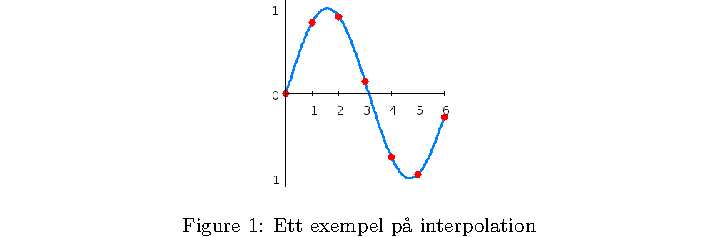
\includegraphics[width=\textwidth,clip=true,trim=80 0 80 0]{ex/4/graphicx.pdf}}
		\end{minipage}
		\caption{Koden till vänster inkluderar filen \cli{interpolation.png} i
		\LaTeX-dokumentet och ger det resultat som ses till höger.}
		\label{fig:graphicx}
	\end{figure}
	
	\subsubsection{Rätt format?}
	En nackdel med \pdfLaTeX{} när det gäller \pack{graphicx} är att det inte
	finns särskilt många bildformat som fungerar (dock fler än för gamla
	\LaTeX{}, som bara accepterade \EPS). De enda format som kan inkluderas
	med \pack{graphicx} när man använder \pdfLaTeX{} är \textsc{PNG},
	\textsc{JPEG} och \PDF. Oftast vill man använda \PDF{} för figurer,
	eftersom
	det är det enda vektorbaserade formatet som fungerar, medan man för
	fotografier och dylikt använder \textsc{JPEG}. \textsc{PNG} kan man
	använda då man egentligen bör använda \PDF{} men detta inte är möjligt.
	
	Eftersom många verktyg och programvaror fortfarande sparar filer i
	\EPS-format kan det vara praktiskt att kunna konvertera dessa till ett
	format som fungerar. Detta kan göras med verktyget \cli{epstopdf}, som
	finns tillgängligt på CTAN.
	
	\subsection{Rita med \PGFTikZ}
	Ett lite mer komplicerat sätt att inkludera grafik (men ofta 
	föredelaktigt, eftersom allt innehåll stannar i \TeX-filen) är att använda
	\PGFTikZ, ett paket skrivet för att användas med \pdfLaTeX{} för att rita
	figurer i \LaTeX{}. Med det kan man direkt i sitt \LaTeX-dokument skapa
	enklare figurer som flödesscheman, träd, grafer eller liknande; se exempel
	i figur~\vref{fig:tikz}. Även mer avancerade figurer är möjliga, men att
	förklara hela \PGFTikZ{} tar allt för lång tid för denna introduktion. Den
	intresserade läsaren hänvisas istället till \citeasnoun{Mertz07} som har
	en bra introduktion till ämnet, och \PGFTikZ-manualen \cite{Tantau10} som
	utförligt beskriver hur paketet fungerar.
	
	\begin{figure}[p]
		\centering
		\begin{minipage}{0.95\textwidth} % kod
			\vfil
			\begin{minted}[frame=single]{latex}
\newcounter{d}\setcounter{d}{0}\def\mcolor{SpringGreen}
\begin{tikzpicture}
    \path[coordinate] (0,0) coordinate(A) ++( 60:6cm)
                      coordinate(B) ++(-60:6cm) coordinate(C);
    \draw[fill=Black!\thed!\mcolor] (A) -- (B) -- (C) -- cycle;
    \foreach \x in {1,...,15}{%
        \pgfmathsetcounter{d}{\thed+10}
        \setcounter{d}{\thed}
        \path[coordinate] coordinate(X) at (A){};
        \path[coordinate] (A) -- (B) coordinate[pos=.15](A)
                            -- (C) coordinate[pos=.15](B)
                            -- (X) coordinate[pos=.15](C);
        \draw[fill=Black!\thed!\mcolor]
				(A)--(B)--(C)--cycle;
    }
\end{tikzpicture}
			\end{minted}
			\vfil
		\end{minipage}
		\\[1ex]
		\begin{minipage}{0.95\textwidth} % figur
			\centering
			\newcounter{density}\setcounter{density}{0}
			\begin{minipage}{0.475\textwidth}
			\fbox{\begin{tikzpicture}
			    \path[coordinate] (0,0)  coordinate(A)
			                ++( 60:6cm) coordinate(B)
			                ++(-60:6cm) coordinate(C);
			    \draw[fill=Black!\thedensity!SpringGreen]
							(A) -- (B) -- (C) -- cycle;
			    \foreach \x in {1,...,15}{%
			        \pgfmathsetcounter{density}{\thedensity+10}
			        \setcounter{density}{\thedensity}
			        \path[coordinate] coordinate(X) at (A){};
			        \path[coordinate] (A) -- (B) coordinate[pos=.15](A)
			                            -- (C) coordinate[pos=.15](B)
			                            -- (X) coordinate[pos=.15](C);
			        \draw[fill=Black!\thedensity!SpringGreen]
							(A)--(B)--(C)--cycle;
			    }
			\end{tikzpicture}}
			\end{minipage}\hfil
			\begin{minipage}{0.475\textwidth}
			\caption[Koden ovan tolkas av \PGFTikZ{} och resulterar i den
			itererade triangeln till vänster]{
			Koden ovan tolkas av \PGFTikZ{} och resulterar i den
			itererade triangeln till vänster.
			Fler exempel finns i
			\citeasnoun{Mertz07} och \citeasnoun{Tantau10}. Tack till Alain 
			Matthes för originalkoden\footnote{\url{http://www.texample.net/tikz/examples/rotated-triangle/}}.}
			\label{fig:tikz}
			\end{minipage}
		\end{minipage}
	\end{figure}
	
	%% (end)
	
	%% REFERENSER MED BIBTEX (fold)
	\section{Referenser med \BibTeX}\label{sec:5}
	%% (end)
	
	%% VIDARE LÄSNING (fold)
	\section{Vidare läsning}\label{sec:6}
	
	\subsection{Andra resurser}
	\subsubsection{Böcker och artiklar}
	\subsubsection{Hjälp med specifika problem}
	% TeX.SE!
	
	\subsection{Rekommenderade paket}
	
	\subsection{Tips för stora projekt}
	
	\subsection{Andra \TeX-baserade projekt}
	\subsubsection{Unicode-baserade \XeTeX}
	\subsubsection{Skripta med \hologo{LuaTeX}}
	%% (end)
	
	\let\oldurl=\url\renewcommand\url[1]{\newline{\small\oldurl{#1}}}
	\bibliography{referenser}
	
	\appendix
	%% EN ENKEL MALL (fold)
	\section{En enkel mall}\label{app:1}
	
	%% (end)

	\backmatter 
	\pagestyle{empty}
	\cleardoublepage\hbox{}\newpage
	{ % EXTERNAL BACK PAGE (fold)
		\pagecolor{\frontpagecolor}
		\color{White}
		\frontpagegraphic
		\begin{tikzpicture}[remember picture,overlay]
			\node [anchor=south east,above=2cm,right=-3.75cm] at (current page.south east)
			 			{
\includegraphics[width=3cm]{qrcode.pdf}};
		\end{tikzpicture}
		\normalcolor
		\newpage
		\pagecolor{White}
	} % (end)
\end{document}